\section{実装環境}
\label{env}

本研究では以下の環境で実装及び実行を行う.
\begin{itemize}
  \item DJI Tello edu
  \item Ubuntu 18.04
  \item python 2.7
\end{itemize}

\subsection{DJI Tello edu}

\begin{figure}[htbp]
  \begin{center}
    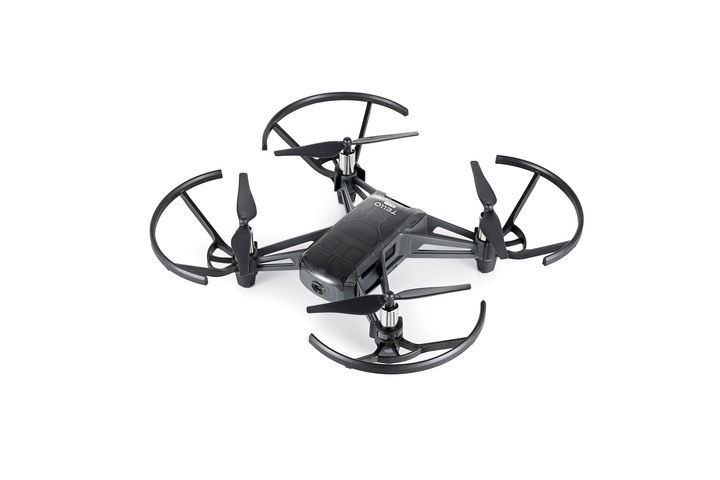
\includegraphics[clip,width=15.0cm]{img/Telloedu.jpg}
    \caption{Tello EDU}
    \label{fig:tello}
  \end{center}
\end{figure}
DJIより発売されている教育向けドローンである\ref{fig:tello}.
公式からSDKが提供されており,多様なAPIを利用可能であり今回は以下のAPIを利用する.
\begin{itemize}
  \item ビデオストリームAPI
  \item コントロールAPI
\end{itemize}

他にミッションパッドと呼ばれるパネルに対しての自己位置推定を行えるAPIや複数機体に同時に制御を行えるようなAPIが用意されている.
また,SDKとしてTelloより送信されるh.264形式の映像ファイルをデコードするC++で記述されたpythonパッケージが提供されている.